\documentclass[tikz,border=5mm]{standalone}
\usepackage{tikz}
\usetikzlibrary{calc}

\begin{document}
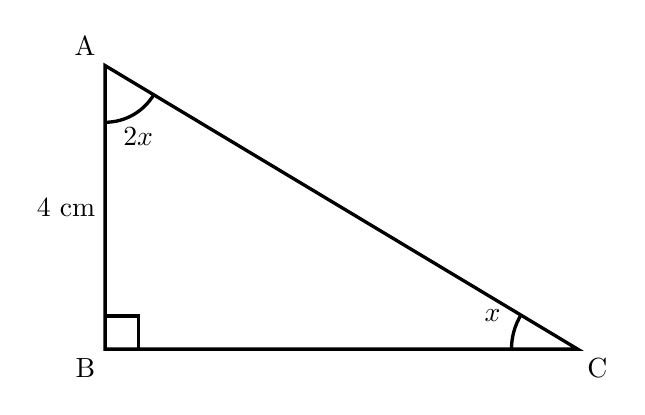
\begin{tikzpicture}[scale=1.2]

% Define vertices
\coordinate (A) at (0,3);
\coordinate (B) at (0,0);
\coordinate (C) at (5,0);

% Draw triangle ABC
\draw[very thick] (A) -- (B) -- (C) -- cycle;

% Draw right angle mark at B
\draw[very thick] (B) ++(0.35,0) -- ++(0,0.35) -- ++(-0.35,0);

% Angle arc at A (2x)
\draw[very thick] ($(A)+(0,-0.6)$) arc[start angle=-90, end angle=-30, radius=0.6];
\node at ($(A)+(0.35,-0.75)$) {\normalsize $2x$};

% Angle arc at C (x)
\draw[very thick] ($(C)+(-0.7,0)$) arc[start angle=180, end angle=149, radius=0.7];
\node at ($(C)+(-0.9,0.35)$) {\normalsize $x$};

% Vertex labels
\node[above left] at (A) {A};
\node[below left] at (B) {B};
\node[below right] at (C) {C};

% Side label (4 cm)
\node[left] at ($(A)!0.5!(B)$) {4 cm};

\end{tikzpicture}
\end{document}